\chapter{КОНСТРУКТОРСКИЙ РАЗДЕЛ}


\section{Используемые технологии}

Одной из трудных задач является исследование доступных технологий. Каждая технология охватывает широкий спектр знаний, поскольку они являются передовыми технологиями, и в прикладных алгоритмах существует математическая поддержка. Конечно, знание теоретических основ важно, но в то же время необходимо проверить, что есть инструменты, которые служат основой проекта. Мы искали доступные технологии и которые мы сейчас представляем.

ProductionIO \cite{predictionio} выбирается в качестве сервера Machine Learning Server с открытым исходным кодом, поскольку он облегчает задачу разработки приложений на основе Spark и многих других решений для больших данных.

Мы выбираем «Apache PredictionIO» в качестве сервера с открытым исходным кодом для создания прогнозирующего движка, чтобы можно было разработать следующий:

\begin{enumerate}
	\item быстро создавать и развертывать движок в качестве веб-сервиса для производства с настраиваемыми шаблонами;

	\item отвечать на динамические запросы в режиме реального времени после развертывания в качестве веб-службы;

	\item систематически оценивать и настраивать несколько вариантов двигателей;

	\item унифицировать данные с нескольких платформ в пакетном режиме или в режиме реального времени для всесторонней прогностической аналитики;

	\item ускорить моделирование машинного обучения с систематическими процессами и заранее подготовленными оценочными мерами;

	\item библиотеки поддержки обучения и обработки данных, такие как Spark MLLib и OpenNLP;

	\item внедрять модели машинного обучения и плавно включать их в свой двигатель;

	\item упростить управление инфраструктурой данных.
\end{enumerate}

\begin{figure}[h]
  \centering
  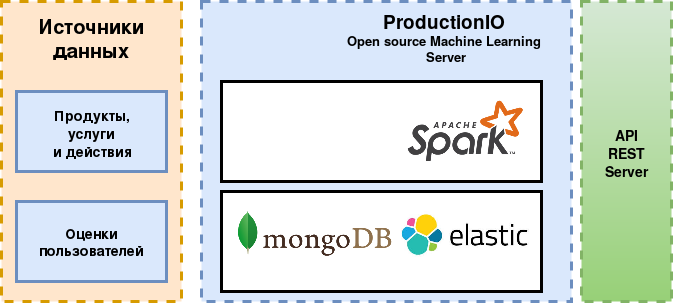
\includegraphics[scale=0.65]{predictionio.png}
  \caption{PredictionIO topology}
  \label{image:alg_timer}
\end{figure}

Apache PredictionIO установлен как полный стековый учебный стек, в комплекте с Apache Spark, MLlib, HBase, Spray и Elasticsearch, который упрощает и ускоряет масштабируемое управление инфраструктурой машинного обучения.

\newpage
\section{Topology}

Наша система рекомендаций разделена на три основных модуля:

\begin{enumerate}
\item Dataset Loader: этот подмодуль загрузит набор данных из Интернета, обработает и сохранит его в наших двух основных хранилищах данных (MongoDB и ElasticSearch).
\item Рекомендательный тренер: все рейтинги, хранящиеся в БД предыдущим модулем, будут использоваться для создания модели совместной совместной работы и предварительного расчета рекомендаций для всех пользователей и продуктов, которые затем будут храниться в MongoDB.
\itemР екомендательный сервер: используя небольшой сервер REST, мы отправим рекомендации для запросов MongoDB и ElasticSearch.
	
\end{enumerate}

Системная топология состоит из распределенной системы обработки информации со следующими задействованными частями: один или несколько экземпляров сервера событий и его механизмы, которые объединяются через API-Rest в центральный API. Центральный API или API «Frontend» - это тот, который взаимодействует с пользователями (веб-браузер, приложение и т. Д.). На первом этапе будет интересна только веб-версия.

\begin{figure}[h]
  \centering
  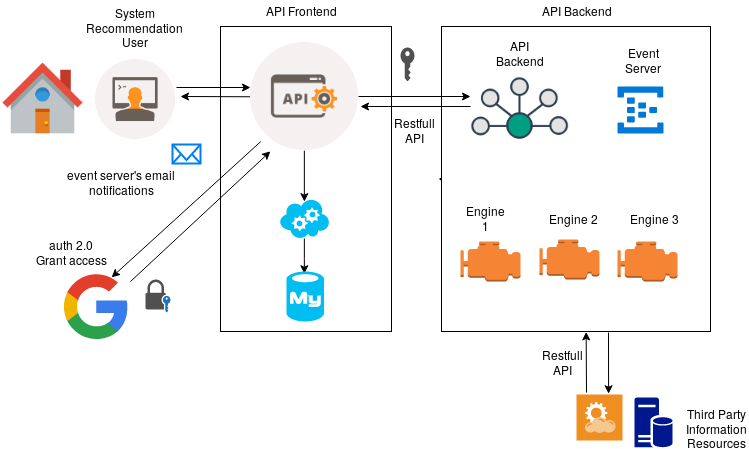
\includegraphics[scale=0.65]{topo2.png}
  \caption{Выбранная топология системы - это микросервисы}
  \label{image:alg_timer2}
\end{figure}


\section{Имплементацион 3 ступени архитектуры}

Три шага в общей архитектуре рекомендательная Системы :
\begin{itemize}
	\item Получение данных
	\item  Предварительно рассчитать
	\item  Получить
\end{itemize}


\textbf{Шаг 1: Проглатывание (Получение данных)}. 
Каждой рекомендуемой системе нужны данные о товарах и пользователях для работы.
\begin{itemize}
	\item Каталог предметов: информация о предметах. Ежедневно / ежечасно обновляется.
	\item Оценки пользователей: неявные или явные оценки генерируются в непрерывном потоке данных.
\end{itemize}


\textbf{Шаг 2: предварительный расчет}.
Рекомендатор Системные недостатки:
\begin{itemize}
	\item Задержка - ключевой фактор в любом сервисе персонализации.
	\item Вычислить рекомендации точно в срок очень дорого и медленно.
\end{itemize}

Наилучшим подходом является предварительный расчет Рекомендаций:
\begin{itemize}
	\item Content Based: современные индексы хранят данные так, что выполнение запросов на поиск выполняется быстро.
	\item Совместная фильтрация: подготовьте модель ALS и предварительно вычислите реквизиты для существующих пользователей и элементов.
\end{itemize}

\textbf{Шаг 3: Получить}. 
Когда запрашиваются рекомендации, просто:
\begin{itemize}
	\item Content Based: создайте запрос, и он будет выполнен индексом.
	\item Collaborative filtering: прочитайте БД для предварительно рассчитанных рекомендаций.
	\item Гибридные подходы: просто попросите несколько источников и объедините результаты.
\end{itemize}



\begin{figure}[h]
  \centering
  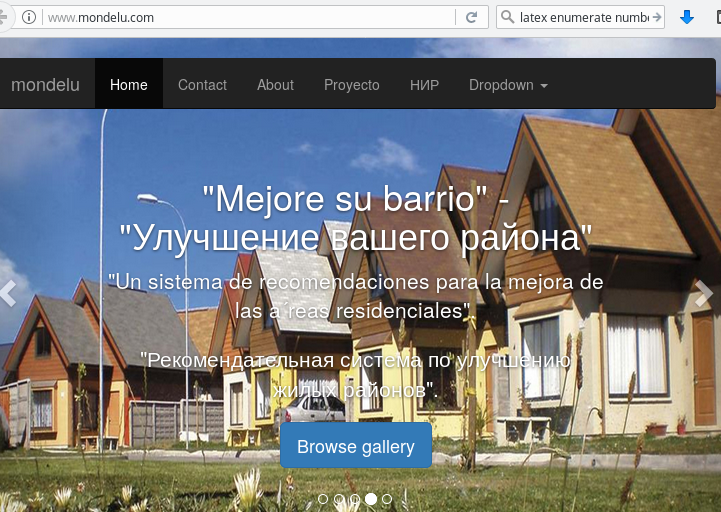
\includegraphics[scale=0.79]{mondelu.png}
  \caption{Test site}
  \label{image:alg_timer3}
\end{figure}

\section{Алгоритмы для рекомендательной системы}

Были выбраны по крайней мере две альтернативы алгоритмов рекомендации. Apache Spark предоставляет различные API-интерфейсы, в этом случае Java API был протестирован в индивидуальной конфигурации на хостинге «DigitalOcean», получив плохие результаты с точки зрения производительности (согласно PredictionIO, требуется минимальная конфигурация 16 ГБ ОЗУ) , В качестве второй альтернативы мы попробуем экземпляр Amazon-EC2 \cite{ec2}(дорогое решение), но только с целью тестирования этих алгоритмов.

\subsection{Алгоритм "K-neighbours" или на основе сходства}

Он будет работать с классом класса «Neighbor», который содержит основной метод программы, который отвечает за вызов остальных классов для выполнения необходимых вычислений. Он также содержит метод для возврата наибольшего идентификационного номера элементов, необходимого для вычисления сходства косинусов.

Он также содержит метод, называемый collectData (), который по пути файла в HDFS читает данные, содержащиеся в нем, и возвращает их в JavaPairRDD, то есть расширение типа ключа / значения RDD, Абстракция искровых объектов. Возвращаемый JavaPairRDD имеет ключевую пару пользователя и в качестве значения содержит элемент и квалификацию (Spark позволяет группировать объекты в одном с классами Tuple2, Tuple3, Tuple4 ...), который связывает пользователя и конкретные элементы, то есть рейтинг, который пользователь дал этому пункту (если он это сделал). Как только эта информация была получена из файла, фильтрация выполняется одним и тем же методом, чтобы ограничить количество пользователей, которые будут участвовать в системе рекомендаций; остальные будут проигнорированы. Это делается для проведения тестов путем изменения количества пользователей и сравнения полученных данных.

После получения сходства между пользователями он выполняет фазу агрегации по рейтингам «соседних» пользователей каждого из них, чтобы получить прогноз рейтинга, который пользователь предоставит каждому элементу.

В MapReduce повторение всех элементов RDD является очень дорогостоящей операцией, поскольку оно поддерживает большой объем данных. Для решения таких проблем, как расчет средних значений пользователей или агрегирование рейтингов, используются восстановительные методы, такие как combByKey, реализация, предоставляемая Spark. Этот метод требует в качестве параметров трех функций: одного из творений, другого дополнения и другого слияния. С первым создается вспомогательный объект указанного типа, при этом к нему добавляются второстепенные элементы, а с третьим объединяются элементы разных объектов (вычисления выполняются параллельно и, следовательно, создается несколько объектов, которые затем они должны собраться).
\subsection{Алгоритм, основанный на тенденциях}

Через класс «Trends», который является основным классом программы, который собирает данные из файла HDFS и управляет вызовом остальным классам. Для получения входных данных он работает так же, как и класс «Соседи» алгоритма, основанного на сходстве.

\subsection{Сравнение альтернатив}

Для этого проекта тестируются по крайней мере два алгоритма, которые позволят в короткие сроки провести дорогостоящие операции. Более конкретно, алгоритм, основанный на «тренде», позволяет проводить миллионы медиа-операций всего за одну секунду.

Сравнивая алгоритм «на основе тенденций» с алгоритмом «K-соседей», оба алгоритма, в которых один имеет более низкую производительность, но лучшую точность данных, а другой, наоборот, должны быть исправлены в ситуации, в которой она предназначена чтобы иметь возможность выбрать один из двух.

С одной стороны, алгоритм, основанный на сходстве или алгоритме соседнего K, имеет очень низкую производительность. Для 8000 пользователей (показатель намного ниже, чем у реальной системы) для выполнения рекомендаций требуется 2 часа. Невозможно использовать его в режиме реального времени, поэтому единственным жизнеспособным выходом для алгоритма, основанного на сходстве, было бы выполнять вычисления в автономном режиме, а затем предлагать их пользователям. Недостатком этого способа предоставления результатов является то, что последние квалификации, которые были сделаны пользователями, не будут учитываться, и хорошие результаты алгоритма с точки зрения уверенности в предсказаниях будут уменьшаться по этой теме.

С другой стороны, алгоритм, основанный на тенденциях, предлагает гораздо лучшие результаты с точки зрения времени. Для системы с 8000 пользователями она рассчитывает прогнозы за 2 минуты, но даже при этом недопустимо ждать пользователя в течение 2 минут (или более) при расчете прогнозов. Он также должен быть выполнен в автономном режиме, но, в отличие от предыдущего алгоритма, он может работать более часто и предлагать более современные данные и, следовательно, уменьшать недостаток, который он имеет с точки зрения точности предсказаний относительно алгоритма, основанного на сходстве.
Выбор того или иного алгоритма будет зависеть от характера системы рекомендаций, которую вы хотите реализовать.

\begin{lstlisting}[language=Scala, caption={Class K Neigborhoods},label=kneigh]
    import org.apache.spark.HashPartitioner;
    import org.apache.spark.SparkConf;
    import org.apache.spark.api.java.JavaPairRDD;
    import org.apache.spark.api.java.JavaSparkContext;
    import org.apache.spark.api.java.function.Function;
    import org.apache.spark.api.java.function.PairFunction;
    import scala.Tuple2;
    import java.util.*;
    public class Neighbours {
        // variables de contexto
        static SparkConf conf;
        static JavaSparkContext sc;

        static public int maxItem (final JavaPairRDD<Integer, Tuple2<Integer, Double>> ratings) {
        return ratings.map(x -> x._2()._1()).top(1).get(0);
        }

        static public JavaPairRDD<Integer, Tuple2<Integer, Double>> collectData(String path, final Integer max){
        return sc.textFile(path)
            .mapToPair(s -> {
                List<String> separated = Arrays.asList(s.split("::"));
                Integer u = Integer.parseInt(separated.get(0)); //usuario
                Integer i = Integer.parseInt(separated.get(1)); // ítem
                Double r = Double.parseDouble(separated.get(2)); // rating
                return new Tuple2(u, new Tuple2(i, r));
            })
            .filter(new Function<Tuple2<Integer, Tuple2<Integer, Double>>, Boolean>() {

            public Boolean call(Tuple2<Integer, Tuple2<Integer, Double>> x) {
                return (x._1().compareTo(max) <= 0); // limitar el número de usuarios
            }   
    });
}


\end{lstlisting}

\newpage
\begin{lstlisting}[language=Scala, caption={Class Trends},label=trends]
    import org.apache.spark.HashPartitioner;
    import org.apache.spark.SparkConf;
    import org.apache.spark.api.java.JavaPairRDD;
    import org.apache.spark.api.java.JavaSparkContext;
    import org.apache.spark.api.java.function.*;
    import scala.Tuple2;
    import java.util.Arrays;
    importjava.util.List;
    public class Trends {
        // variables de contexto
        static SparkConf conf;
        static public JavaSparkContext sc;
        static public JavaPairRDD<Tuple2<Integer,Integer>, Double> collectData(String path, final Integer maxUser){ 
      
            return sc.textFile(path)
                .mapToPair(s -> {
                    List<String> separado = Arrays.asList(s.split("::"));
                    Integer user = Integer.parseInt(separado.get(0));
                    Integer item = Integer.parseInt(separado.get(1));
                    Double r = Double.parseDouble(separado.get(2));
                    return new Tuple2(new Tuple2(user, item), r);
            }).filter(new Function<Tuple2<Tuple2<Integer, Integer>, Double>, Boolean>() {
                public Boolean call(Tuple2<Tuple2<Integer, Integer>, Double> x) {
                    return (x._1()._1().compareTo(maxUser) <= 0); // 1000 usuarios
                }
            });
}
\end{lstlisting}

\newpage

\begin{lstlisting}[language=Scala, caption={Class CosineSimilarity},label=trends]

import org.apache.spark.HashPartitioner;
import org.apache.spark.api.java.JavaPairRDD;
import org.apache.spark.api.java.JavaRDD;
import org.apache.spark.api.java.JavaSparkContext;
import org.apache.spark.api.java.function.PairFunction;
import org.apache.spark.mllib.clustering.VectorWithNorm;
import org.apache.spark.mllib.linalg.BLAS;
import org.apache.spark.mllib.linalg.Vector;
import org.apache.spark.mllib.linalg.Vectors;
import scala.Tuple2;

public class CosineSimilarity {
    final JavaPairRDD<Integer, Tuple2<Integer, Double>> ratings;


    public CosineSimilarity (JavaPairRDD<Integer, Tuple2<Integer, Double>> r) {
        ratings = r.cache();
    }



    public JavaPairRDD<Tuple2<Integer, Integer>, Double> computeSimilarity (final Integer maxItem){
        // entrada: <<usuario1, vector1>, <usuario2, vector2>>
        // salidas: <usuario1, usuario2>, similitudCoseno
        PairFunction<Tuple2<Tuple2<Integer, Vector>, Tuple2<Integer, Vector>>,
            Tuple2<Integer, Integer>, Double> compute =
            (x) -> {
            final Double den1 = (new VectorWithNorm(x._1()._2())).norm();
            final Double den2 = (new VectorWithNorm(x._2()._2())).norm();
            Double num = BLAS.dot(x._2()._2(), x._1()._2());
            return new Tuple2 (new Tuple2(x._1()._1(), x._2()._1()), (num / (den1 * den2)));

            };
    JavaRDD<Tuple2<Integer, Vector>> vectors = ratings
            .groupByKey(new HashPartitioner(7))
            .map(r -> new Tuple2(r._1(), Vectors.sparse(maxItem+1, r._2()))); // <usuario, vectorRatings>
    
    return vectors
            .cartesian(vectors) // <<usuario1, vectorRatings1>, <usuario2, vectorRatings2>>
            .filter(x -> x._1()._1() != x._2()._1()) // user1 != user2
            .mapToPair(compute); // <<user1, user2>, similitud>
    }
}
\end{lstlisting}


